%!TEX root = ../dissertation.tex
\section{The Cellular Model}
We selected two mono-cultures of human neuronal cells for subsequent experiments: \acs{la2} and \acs{la5}. During the selection process, multiple options were considered. Multicellular models would, in principle, allow disentanglement of the functions of distinct cell types, for instance glia and neurons. This could be achieved by \emph{in vivo} or \emph{ex vivo} approaches in rodents. However, our diseases of interest (Section \ref{sec:intro:diseases}) display a noticeable lack of transferability from lower mammals to human(cite). Alternatively, co-cultures of human cells in mono-layer or as 3D-culture have been proposed, but these still lack experimental stability.

\subsection{The SH-SY5Y Neuroblastoma Cell Line}
A prominent example of human neuronal cell culture used in the identification and elucidation of cholinergic processes is the immortalised neuroblastoma cell line SH-SY5Y.\cite{Biedler1978} Derived from its parent line SK-N-SH, an adrenergic neuroblastoma,\cite{Biedler1973} it expresses ample amounts of \textit{\ac{ache}}, and thus had become a work horse in many cholinergic fields, such as Alzheimer's Disease (which is treated with \ac{achep} inhibitors), pesticide development, and warfare(cite). However, in spite of its usefulness for processes involving \textit{\ac{ache}}, it turned out a less than optimal choice for the study of molecular events surrounding \textit{\ac{chat}} and \textit{\ac{slc}}, as it barely expresses both genes(cite), and cannot be coerced to elevate \textit{\ac{chat}} expression by the usual differentiation techniques (own experimentation, data not shown). Thus, for the questions asked in this chapter of the dissertation, SH-SY5Y does not qualify as adequate representation of a »cholinergic neuron«.

\subsection{The LA-N Neuroblastoma Cell Lines}
Following the elimination of SH-SY5Y as a suitable subject, a literature search for candidates representing a cholinergic neuronal transcriptome revealed, among others, representatives of the LA-N neuroblastoma cell lines developed by R.C. Seeger around 1980.\cite{Seeger1977, Seeger1982} Neuroblastoma is a form of neuronal cancer often affecting small children, and, consequently, the two cell lines used in my experiments are immortalised biopsies of a 3 year old girl (\acs{la2}\cite{Seeger1977}) and of a 4 month old boy (\mbox{\acs{la5}}\cite{Seeger1982}). The decision to use \ac{la2} as initial cellular model was influenced by three factors: it is well described in literature, although most studies had been published in the 1980s and 90s; it expresses substantial amounts of \textit{\ac{chat}} and \textit{\ac{slc}}(cite); and it responds to neurokine-mediated differentiation by assuming a neuronal morphology accompanied by further elevation of \textit{\ac{chat}} and \textit{\ac{slc}} expression. \ac{la5} was not nearly as well described as \ac{la2}, but later added to the experimental roster because of the complementary sex and hints towards cholinergic differentiation under retinoic acid.\cite{Hill1997}

\begin{method}

\subsection{Culture}

\ac{la2} and \ac{la5} are very similar in their culture requirements. They have comparatively high duplication times, which can be lowered by using certain conditions that affect medium composition, nutrition, and CO\textsubscript{2} content. The cells were acquired at DSMZ (Braunschweig, Germany), which recommends keeping them in a 50:50 mixture of \ac{dmem} and \ac{rpmi}, with 20\% \ac{fcs} added. Sometimes, recommendations also suggest Leibovitz's L-15 medium, which is specifically designed for low CO\textsubscript{2} conditions, and others have suggested increased CO\textsubscript{2} levels inside the incubator. A combination of the DSMZ-recommended medium with 8\% CO\textsubscript{2} atmosphere inside a 37°C incubator to accelerate growth to a degree that the cells could be split 1:3 to 1:4 in a weekly cycle. This protocol was used for all further experiments, which were performed between splits 2 to 8 after thawing of a batch from -80°C. All handling during maintenance and experimentation was performed under a laminar flow hood.

\subsection{Differentiation}

Neuronal differentiation of neuroblastoma cell lines has been performed in many instances, utilising a wide variety of differentiation agents such as the very general retinoic acid or 5-bromo-uracil, or very specific reagents, such as the neurokines \ac{il}-6 and \ac{cntf}(cite). LA-N cells have also been described to react to a selection of these substances; however, due to our elevated interest in neurokine mechanisms, we opted for a neurokine-based differentiation protocol. In personal communication, James McManaman revealed that the »\textit{\ac{chat}} development factor« that he had discovered\cite{McManaman1988} was, in fact, \ac{cntf}, which had never been published. Additionally, of the neurokines used for differentiation purposes, \ac{cntf} is best described in literature and easily acquired in dried form from Merck (formerly SigmaAldrich, Darmstadt, Germany). \ac{cntf} was resuspended in pure water to a concentration of \SI{25}{\micro\gram\per\milli\litre} and stored for experimentation in aliquots at -20°C.

LA-N cells are very sensitive to repeated temperature changes (or other handling-related disturbances), which resulted in increased amounts of apoptotic cells following repeated removal from the incubator after seeding or medium changes during the experiment (Lobentanzer, not published). For this reason, the differentiation reagent was only added once, 24h after initial seeding of the cells, and further disturbances avoided until the time of lysis. For the maximum duration of the experiments, 120h from seeding until lysis, the initially supplied medium was sufficient for survival.

Differentiation was performed in regular growth medium without changes in \ac{fcs} content, and \ac{cntf} was added to the medium after an initial growth period of 24h. Cells were seeded into 12-well plates at approximately \num{200000} cells/well, with 1 ml of growth medium. To determine the optimal amount of \ac{cntf} for differentiation, time-dose experiments were perfomed for both cell lines in a range from \SIrange{1}{100}{\nano\gram\per\milli\litre} for several time points during four days. Here, we discovered the first pharmacological difference between \ac{la2} and \ac{la5}: the maximum of their cholinergic response to neurokine stimulation (i.e., an elevation in \textit{\ac{chat}} and \textit{\ac{slc}} transcription) occurs at different concentrations of \ac{cntf}. While \ac{la2} cells respond most strongly to \SI{100}{\nano\gram\per\milli\litre}, \ac{la5} cells show an »inverted u«-type dose response with a maximum around \SI{10}{\nano\gram\per\milli\litre} \ac{cntf} (Fig.\,\ref{fig:time-dose}). James McManaman, who studied LA-N differentiation thoroughly in the 1990s,\cite{McManaman1991} believes both lines to respond in an »inverted u«-type manner (personal communication); thus, in all likelihood the \ac{la2} response would also diminish at \ac{cntf} concentrations significantly higher than \SI{100}{\nano\gram\per\milli\litre}. Also, CNTF concentrations could likely be significantly lowered by removal of the high amount of \ac{fcs} in the medium, however, that would require the use of a special serum-free medium, which would have to be established up front, and may have other, unforeseen consequences. Regardless, \ac{cntf} concentrations around \SI{100}{\nano\gram\per\milli\litre} (i.e., pico- to nano-molar) still are well within the physiological range of concentrations that the mammalian brain is able to reach by paracrine secretion via, e.g., astrocytes.\cite{Sun2016}\todo{combine fig 3.4, 3.5}\todo{vacht qpcr figure?}

\end{method}

\begin{figure}
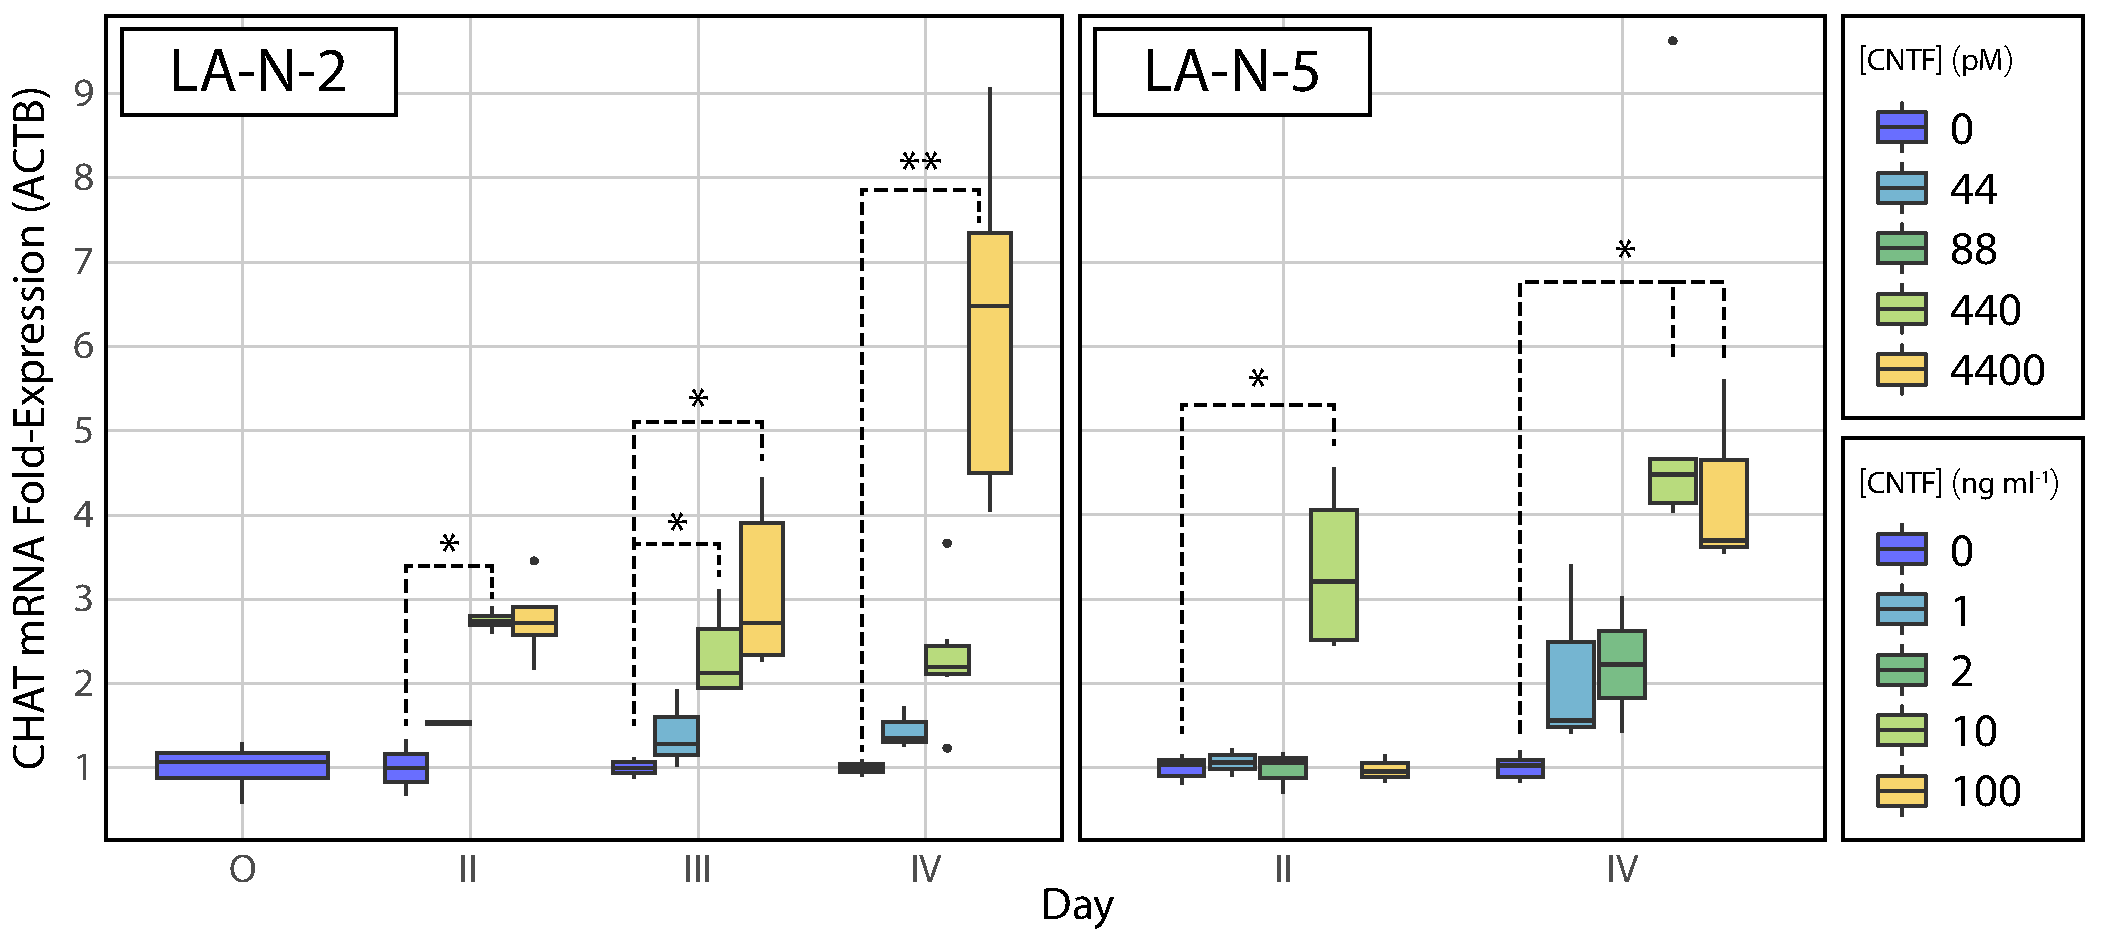
\includegraphics[width=\textwidth]{figures/time-dose}
\caption[Time-dose curve, LA-N-2 and LA-N-5.]{\textbf{Time-dose curve of CNTF-mediated differentiation of LA-N-2 and LA-N-5.} Cells were stimulated with varying doses of CNTF, and lysed at various time points to determine CHAT mRNA levels via qPCR. Expression ($\Delta\Delta{C}_t$) was normalised to housekeeping genes (ACTB, GAPDH, RPLP0) and to control sample without CNTF to determine fold-changes. LA-N-5 reacts strongest to a concentration of \SI{10}{\nano\gram\per\milli\litre}, while LA-N-2 reacts strongest to \SI{100}{\nano\gram\per\milli\litre}. *: p < 0.05, **: p < 0.001
\label{fig:time-dose}}
\end{figure}

\begin{method}

To study the small RNA dynamics following \ac{cntf} exposure of \ac{la2} and \ac{la5}, the experiment was stopped at 4 time points and the cells were quickly lysed \textit{in situ} to preserve total RNA in that state: for the quick, immediate-early-like phase, at 30 and 60 minutes after the addition of \ac{cntf}, and, for the long-term effects of differentiation, at 48 and 96 hours after the addition of \ac{cntf} (Fig.\,\ref{fig:timepoints}, from Lobentanzer \textit{et al.}\cite{Lobentanzer2019a}). Each time point was controlled by a pseudo-treated (using pure water) culture from the same batch that had been seeded at the same time as the experimental group. In the final series used for the parallel sequencing of \ac{la2} and \ac{la5}, all experiments were carried out in quadruplicates. 

\end{method}

\begin{figure}
\centering
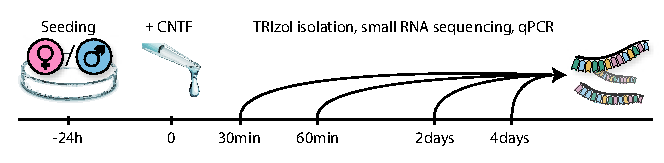
\includegraphics[width=0.8\textwidth]{figures/timepoints}
\caption[LA-N-2 / LA-N-5 Differentiation Timeline.]{\textbf{LA-N-2 / LA-N-5 Differentiation Timeline.} Cells were seeded at $\smallsim$\e{2}{5} cells/well in a 12-well-plate. After 24h, CNTF was added to the existing medium as quickly as possible to avoid disturbance. Cells were lysed \textit{in situ} at time points 30 minutes, 60 minutes, 48 hours, and 96 hours using TRIzol for downstream RNA processing.
\label{fig:timepoints}}
\end{figure}

\begin{method}

\subsection{RNA Isolation}

Total RNA was isolated using TRIzol (ThermoFisher Scientific), essentially as suggested by the manufacturer, with slight changes to the protocol to enrich small RNA species. The cells, growing in a monolayer in 12-well-plates, were cleared of medium, washed two times with \SI{500}{\micro\litre} of cell culture grade \ac{pbs} (Gibco), and immediately suspended in \SI{1}{\milli\litre} of TRIzol, pipetting up and down until visibly dissolved. After incubation for 5 minutes at room temperature, the samples were stored in -20°C for short periods of time until RNA isolation.

TRIzol-suspended lysates (\SI{1}{\milli\litre}) were added to RNA-separation centrifuge tubes (PhaseMaker Tubes, ThermoFisher Scientific), adding \SI{200}{\micro\litre} of pure chloroform and mixing vigorously for 15 seconds. After two minutes, the mixture was centrifuged at \SI{12000}{\g} and 4°C for 15 minutes, and the upper, watery phase containing the RNA was extracted. This was mixed with approximately 2 parts of pure ethanol and incubated for 10 minutes at room temperature to precipitate the RNA. The precipitate was spun at \SI{12000}{\g} and 4°C for another 10 minutes, and the supernatant discarded. The pellet was washed with 85\% ethanol (vortexed briefly) and centrifuged again for 5 minutes at \SI{7500}{\g} and 4°C.

After the final centrifugation step, the samples were transferred to the laminar flow hood, and air dried after removal of most of the supernatant via micropipettors. The pellet was allowed to dry almost until completion and resuspended in \SIrange{30}{50}{\micro\litre} pure RNase-free water. RNA concentration was measured at a Nanodrop 2000 instrument (ThermoFisher Scientific) and samples were diluted to a uniform concentration of \SI{100}{\nano\gram\per\micro\litre}. Finally, RNA samples were aliquoted according to later purpose and stored at -80°C.

RNA quality was determined by analysis on a 2100 Bioanalyzer instrument (Agilent) using a nano chip and \SI{1}{\micro\litre} of sample; \ac{rin} was near optimal for all samples (>9).

\section{Small RNA Sequencing and Differential Expression Analysis}
\newthought{For the detection and analysis of small RNA species}, \ac{seq} is the current gold standard method. It allows the mapping of a comprehensive transcriptome and thus is vastly superior to small scale and consecutive methods such as \ac{pcr}, and even the larger scale microarrays. Microarrays, while also potentially allowing a »snapshot« of entire transcriptomes, are limited by the predetermined sequences on the chip. \ac{seq}, on the other hand, is not biased towards any structural property of the sample; this is particularly important in the analysis of small RNA species, since their sequences are very variable (\acp{trf}) and still not completely catalogued (\acp{mir}). Assuming an adequate sequencing depth ($\smallgtrsim$\e{1}{6} reads/sample), \ac{seq} allows a comparison of all expressed small RNA species at once, which is immensely helpful when dealing with processes on the combinatorial scale of \ac{mir} regulation.

\subsection{Sequencing} \label{sec:cellculture:sequencing}

For small RNA sequencing, the aliquoted samples were shipped on dry ice to the cooperating institute at the Hebrew University of Jerusalem, the Silberman Institute of Molecular Biology, the laboratory of Prof. Hermona Soreq. \SI{600}{\nano\gram} of total RNA per sample were prepared for sequencing using the NEBNext Small RNA Library Prep Set for Illumina (New England BioLabs). The libraries were multiplexed with coloured barcodes, allowing for sequencing of all 48 samples on one chip. Briefly, this includes ligation of sequencing adapters to both 3' and 5' ends of all (single-stranded) RNA fragments in the sample, followed by 12-15 cycles of reverse transcription to form the RNA library. Ligated and amplified libraries were then size selected via gel electrophoresis on a 6\% Polyacrylamide gel. The band representing small RNA species on the gel was excised and prepared for loading onto the sequencing chip. After loading, the chip was sequenced in a NextSeq 550 series instrument (Illumina) with a read length of 80 \acfp{nt}, single-end. 

The quantity of reads per sample was determined by analysis of the raw fastq files. The read count across all samples before filtering was \e{7.8}{06} $\pm_{SD}$ \e{2.5}{6}, read count after quality filter and adapter removal was \e{6.8}{6} $\pm_{SD}$ \e{2.2}{6} (n = 48); a mean of 87\% of reads remained after filtering, exceeding the recommended minimum amount ($\smallsim$\num{1} million) by 4- to 12-fold (Fig.\,\ref{fig:read-quality-length}\,A). Overall, $\smallsim$326 million reads remained to be passed down to subsequent analyses. Sequencing quality was determined by analysis of the raw reads using the FastQC software(cite). Even before adapter removal and quality filtering, FastQC detected no »reads of poor quality« in any sample. Fig.\,\ref{fig:read-quality-length}\,B gives a representative example of read quality per base (Sample \num{1}).

\end{method}

\begin{figure}[ht]
\centering
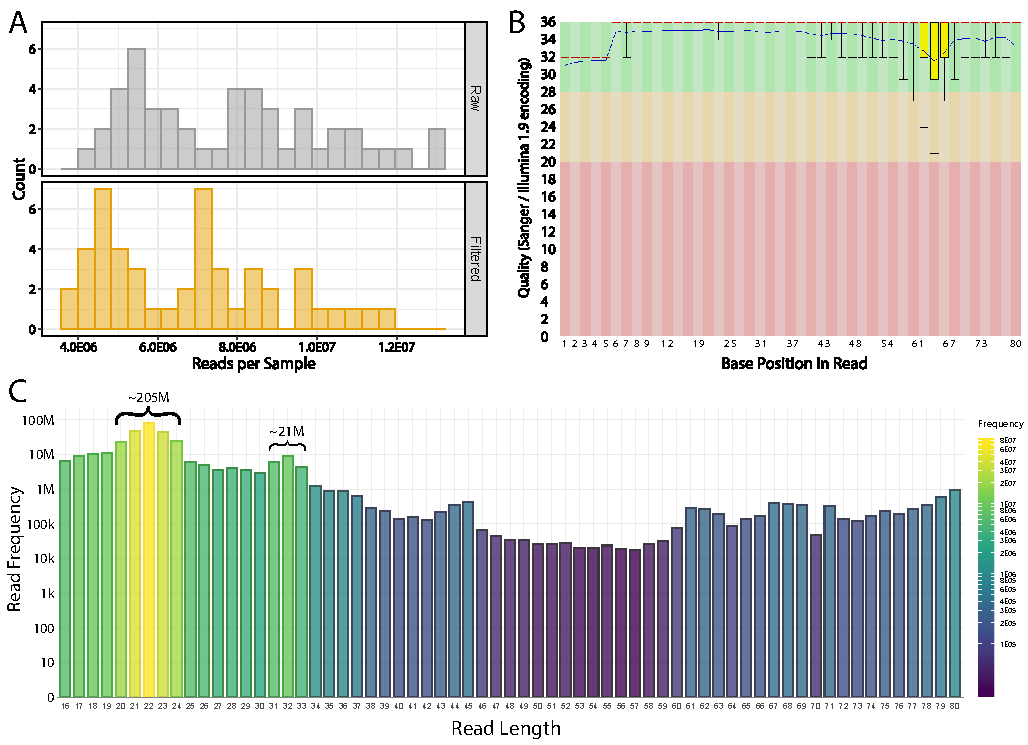
\includegraphics[width=\textwidth]{figures/read-quality-length}
\caption[Small RNA Sequencing - Read Count, Quality, and Length.]{\textbf{Small RNA Sequencing - Read Count, Quality, and Length.} All samples provided near optimal quality. \textbf{A)} Per sample read count had a mean of \e{7.8}{06} $\pm_{SD}$ \e{2.5}{6} in raw samples (top) and \e{6.8}{6} $\pm_{SD}$ \e{2.2}{6} after quality filtering and adapter removal (bottom). 87\% of reads were retained after filtering, with samples spanning read count values between 4 and 12 million. \textbf{B)} Representative example of quality score per base position in the sequencing (FastQC output of sample \num{1}). Quality scores are always near the optimum, with a characteristic slight dip around nt 65. This occurs in all samples and is likely a technical result of the sequencing process. Possibly, it reflects the most common adapter ligation position after size selection of the RNA pool. \textbf{C)} Read length was determined for every one of the $\smallsim$326 million reads. Nearly 80 million reads have a length of 22 nt, and the peak from 21 to 24 nt comprises $\smallsim$205 million reads. This represents the bulk of miRNAs, and probably a significant amount of tRFs. The second peak, from 31 to 33 nt, still comprises $\smallsim$21 million reads; these in all likelihood represent the longer tiRNAs. The reads above a length of 33 nt only sum up to an amount of $\smallsim$6 million, and may contain RNA of viral origin, or even mature tRNAs.
\label{fig:read-quality-length}}
\end{figure}

\begin{method}

Raw reads were adapter-trimmed and quality filtered using the flexbar software\cite{Roehr2017} with parameters

\begin{center}\texttt{-a adapters.fa -q TAIL -qf sanger -qw 4 \\-min-read-length 16 -n 1 --zip-output GZ}\end{center} 

The sequence used in the \textit{adapters.fa} file, as recommended by the manufacturer, was $$AGATCGGAAGAGCACACGTCTGAACTCCAGTCAC$$ 

Paired-end sequencing still is superfluous in small \ac{seq}, because none of the common alignment pipelines can use the second (reverse) read, and manual paired alignment does not yield nearly as much benefit as the depth increase in single-end sequencing (the read count per sample effectively doubles). 80 \acp{nt} is the maximum read length possible in our small RNA workflow, and is excessive for the analysis of \acp{mir}. For \aclp{trf}, however, a longer read can yield a more complete picture of expression, since the longer \acp{tirna} can easily reach 40 \acp{nt} in length. Indeed, the read length distribution after adapter removal shows a significant amount of small RNA species exceeding the length possible for \acp{mir} (Fig.\,\ref{fig:read-quality-length}\,C).  \todo{align longer reads to genome? viral?} \todo{discuss in text?}

\end{method}

%\begin{figure}
%\centering
%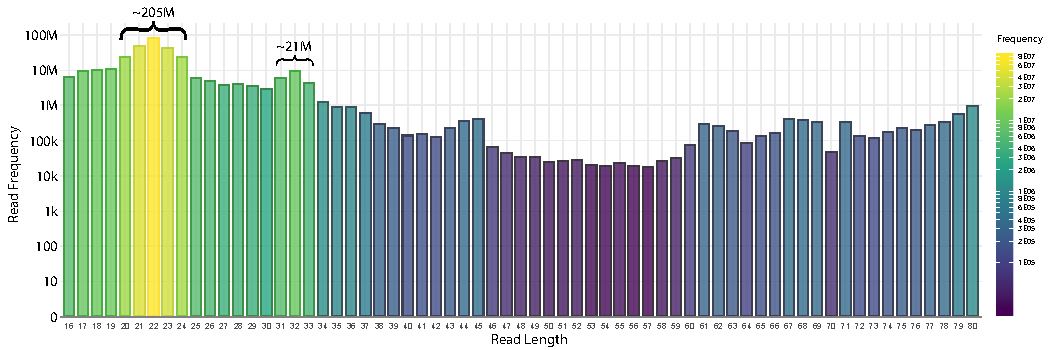
\includegraphics[width=\textwidth]{figures/read-dist-after-flexbar}
%\caption[Small RNA Sequencing - Read Distribution after Trimming and Filtering.]{\textbf{Small RNA Sequencing - Read Distribution after Trimming and Filtering.} Read length was determined for every one of the $\smallsim$326 million reads. Nearly 80 million reads have a length of 22 nt, and the peak from 21 to 24 nt comprises $\smallsim$205 million reads. This represents the bulk of miRNAs, and probably a significant amount of tRFs. The second peak, from 31 to 33 nt, still comprises $\smallsim$21 million reads; these in all likelihood represent the longer tiRNAs. The reads above a length of 33 nt only sum up to an amount of $\smallsim$6 million, and may contain RNA of viral origin, or even mature tRNAs.
%\label{fig:read-dist-after-flexbar}}
%\end{figure}

\begin{method}

\subsection{Sequence Alignment} \label{sec:cellculture:alignment}

For the alignment of \ac{mir} sequences, parts of the miRExpress 2.0\cite{Wang2009} pipeline were used according to the documentation. First, a lookup table for the current miRBase version 21 was created as per the instructions of the authors. The alignment was then performed using the commands \textit{Raw\_data\_parse}, \textit{statistics\_reads}, \textit{alignmentSIMD}, and \textit{analysis}; \textit{Trim\_adaptor} \todo{describe what miRExpress does?} was skipped because the adapters had already been trimmed in the quality filtering step. Additionally, since miRExpress is not accepting of sequences of any length, the raw data was length filtered to include only reads up to a length of 25 \acp{nt} before input into miRExpress. Thus, raw reads were aligned to the miRnome provided by miRBase v21, yielding count tables of mature \acp{mir} and miRNA precursors for each sample. In total, 1913 mature \acp{mir} from miRBase v21 were discovered in the data.

\subsection{Differential Expression Analysis - R/DESeq2} \label{sec:cellculture:deseq}

To determine the effect and dynamics of \ac{cntf}-mediated differentiation of \ac{la2} and \ac{la5}, the expression state of each measured time point was compared to the respective control using the established R package \textit{DESeq2}.\cite{Love2014} \textit{DESeq2} determines differential expression (for gene $i$ and sample $j$) in count-based data by application of a linear regression model to a negative binomial distribution based on a fitted mean $\mu_{ij}$ and a gene-specific dispersion value $\alpha_i$. The mean is derived using a sample-specific »size factor«, $s_j$, and a parameter $q_{ij}$ proportional to the expected true concentration of RNA fragments in the sample. The \textit{DESeq2} differential expression pipeline is composed of the following commands:
\begin{itemize}[noitemsep, leftmargin=.5cm, label={\tiny\raisebox{1ex}{\textbullet}}]
\item \texttt{estimateSizeFactors()} to estimate $s_j$
\item \texttt{estimateDispersion()} to estimate $\alpha_i$
\item \texttt{nbinomWaldTest()} application of a generalised linear model to determine log-fold changes and statistics via the Wald test, using $\mu_{ij} = s_jq_{ij}$ and $log_2(q_{ij}) = x_j\beta_i$.
\end{itemize}
The Wald test, named after Abraham Wald,\cite{Wald1939} is an approach to hypothesis testing that measures the distance between the tested unrestricted estimate and the null hypothesis, using the precision as a weighting factor. The larger the distance between tested values and the null, the more likely the measured values are »true«. \ac{seq} data can be modelled using binomial distributions,\cite{Bullard2010} such as the Poisson distribution, and the difference between two Poisson means (e.g., »treated« vs »control«) can be tested by generalised linear models based on the distributions directly (Poisson regression), Fisher's exact test, or the likelihood ratio test. However, comparative analysis has shown that the Wald test on log-transformed data provides statistical power superior to these other methods,\cite{Chen2011} particularly in lowly expressed fragments. The design formula for the linear regression was applied to \ac{la2} and \ac{la5} separately as a simple factor combination of condition and time point: $$y \smallsim condition\_time$$

To reduce the noise introduced by the high variance in low-count genes while preserving large, »real« differences, the authors propose the »shrinkage« of log-fold changes to avoid arbitrary low-cut filtering at a predefined expression (count) value. Multiple variants are available; for \ac{mir} data, the adaptive algorithm »apeglm«\cite{Zhu2019} (adaptive t prior shrinkage estimator) yielded sensible results (see Fig.\,\ref{fig:apeglm-comp-la2d4}).

\end{method}

\begin{figure}[ht]
\centering
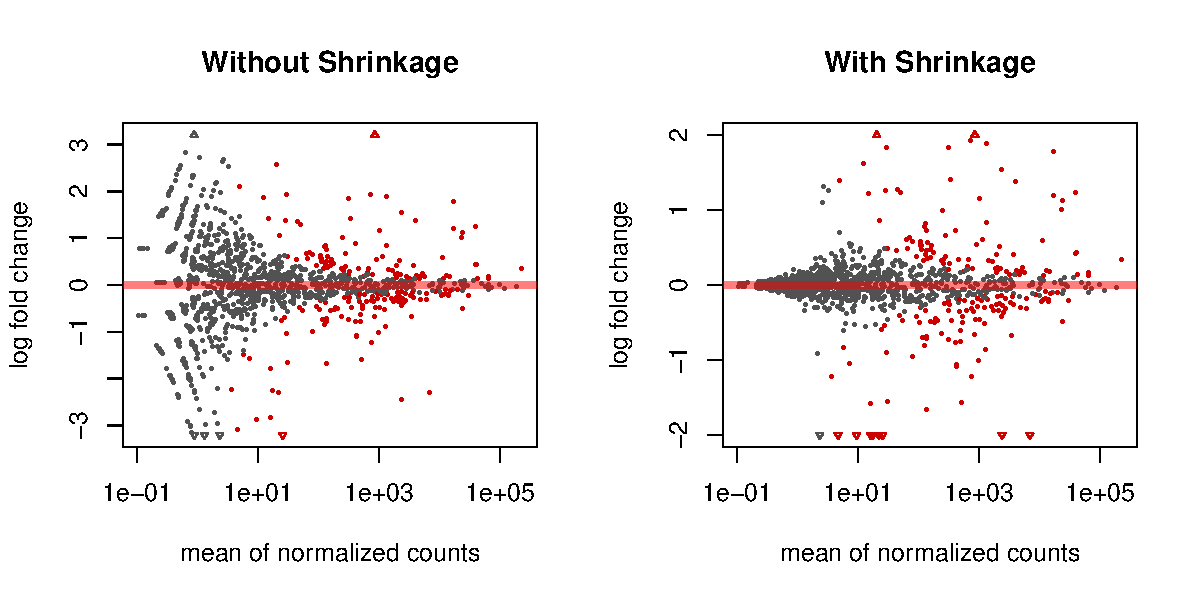
\includegraphics[width=\textwidth]{figures/apeglm-comp-la2d4}
\caption[MD Plot Shrinkage Comparison.]{\textbf{MD Plot Shrinkage Comparison.} A mean-difference plot (MD Plot) is a plot of log-intensity ratios (differences, »M-values«) versus log-intensity averages (means, »A-values«); it is synonymous with »MA Plot«. The \textit{DESeq2} function \textit{plotMD} shows the fold changes attributable to a given variable over the mean of normalised counts for all the samples in the data set. Points will be coloured red if the adjusted p value is less than 0.1. Points which fall out of the window are plotted as open triangles pointing either up or down. The left plot is generated from the standard linear model, the plot on the right is corrected by the »apeglm« algorithm\cite{Zhu2019} to reduce noise in the low-count fragments (data from \ac{la2} \ac{cntf} vs control on day 4).
\label{fig:apeglm-comp-la2d4}}
\end{figure}

\subsection{microRNA Dynamics in CNTF-mediated Cholinergic Differentiation of LA-N-2 and LA-N-5}
Differential expression analysis performed in this manner yielded 490 \ac{de} \acp{mir} across all groups, with characteristic distributions between cell lines and time points. The raw data and processed counts were deposited to \ac{ncbi} \ac{geo}, accession GSE132951. An earlier sequencing experiment (deposited as GSE120520), which was similar in principle, but only comprised three biological replicates and only \ac{la2}, reproduced 80\% of \ac{de} \acp{mir} in the newer \ac{la2} samples. Considering the general reproducibility of \ac{seq} and the lower replicate number, 80\% is an excellent substantiation of the result. About 25\% of miRNAs predicted in single-cell permutation targeting analysis (see Fig. \ref{fig:singlecell}\,E) were found DE in LA-N-2 and LA-N-5 (Fig. \ref{fig:cc-cor-de-perm}\,A) in all three groups, i.e., conserved, primate-specific, and TF-targeting miRNAs.  

\subsubsection{Differential Expression in Both Cell Lines}

%\begin{wrapfigure}{r}{0.5\textwidth}
%  \begin{center}
%    \includegraphics[width=0.48\textwidth]{birds}
%  \end{center}
%  \caption{Birds}
%\end{wrapfigure}

114 mature \acp{mir} were detected as \ac{de} in both cell lines, with some changes similar in both, while others were inverted (Fig.\,\ref{fig:cc-cor-de-perm}\,B). In both cases, however, count-change values (see Box \ref{box:count-change}) correlated highly between the two cell lines (similar: 76 \acp{mir}, Spearman’s $\rho = 0.9066$, p < 2.2E-16; inverted: 38 \acp{mir}, $\rho = 0.9294$, p < 2.2E-16).

\begin{figure}[ht]
\centering
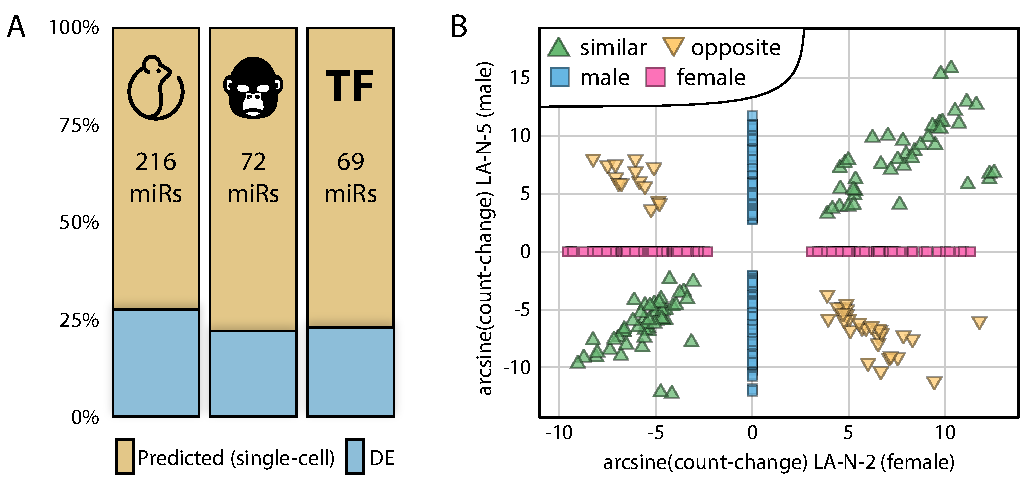
\includegraphics[width=\textwidth]{figures/cc-cor-de-perm}
\caption[Differentially Expressed microRNAs in LA-N-2 and LA-N-5.]{\textbf{Differentially Expressed microRNAs in LA-N-2 and LA-N-5.}
\label{fig:cc-cor-de-perm}}
\end{figure}

\begin{mybox}{The count-change metric}\label{box:count-change}
The frequently used log-fold change metric is not ideally suited for assessing the potential effect of expression changes for individual \acp{mir} because it does not reflect mean expression levels. To determine the absolute change in expression, the count-change metric was introduced, a combination of base mean expression and log-fold change, to weigh DE miRNAs against one another. The count-change is defined as follows: $$CC = (BM \cdot 2^{LFC}) - BM$$
CC: count-change, BM: base mean expression, LFC: log-2-fold-change.

Importantly, by using the base mean expression, count-change correlates directly with sequencing depth. Generalisation, e.g. comparison between two individual experiments, is therefore not straightforward. A normalisation to raw reads would enhance comparability, however, other effects such as fragment distribution and quality aspects may also play a significant role.
\end{mybox}

\subsubsection{Differential Expression Along The Timeline} \label{sec:cellculture:along}
For consistency, from hereon out, time points 30 minutes and 60 minutes will be termed »early«, while 2 days and 4 days will be referred to as »late«. Differential expression was detected in all groups, lending credibility to the rapid changes in expression needed for a \ac{mir} response of the »immediate-early« type. However, the response to long-term \ac{cntf} stimulation was larger in \ac{mir} numbers as well as effect sizes (Fig.\,\ref{fig:timepoints-expr-venn}\,A\&B). Of all early perturbed \acp{mir}, only 3 and 13 \acp{mir} were exclusively perturbed immediate-early-like in \ac{la2} and \ac{la5}, respectively; all others were still \ac{de} after 2 and/or 4 days. In \ac{la2}, the late time points at 2 and, particularly, 4 days showed the greatest perturbation; in \ac{la5}, the picture was more complex (Fig.\,\ref{fig:timepoints-expr-venn}\,C\&D). However, generally, there were large similarities as well as exclusivities between the time points 2 and 4 days in both cell lines. When comparing early and late time points between \ac{la2} and \ac{la5} directly, similarly complex patterns emerged (Fig.\,\ref{fig:timepoints-expr-venn}\,E\&F). Particularly at late time points (Fig.\,\ref{fig:timepoints-expr-venn}\,F), every possible combination of overlap exists. 24\todo{something special?} \acp{mir} were \ac{de} in all late conditions; 107 \acp{mir} were \ac{de} only in \ac{la2}, and 269 \acp{mir} were \ac{de} only in \ac{la5}. \todo{compare most important targets early/late}

\begin{figure} 
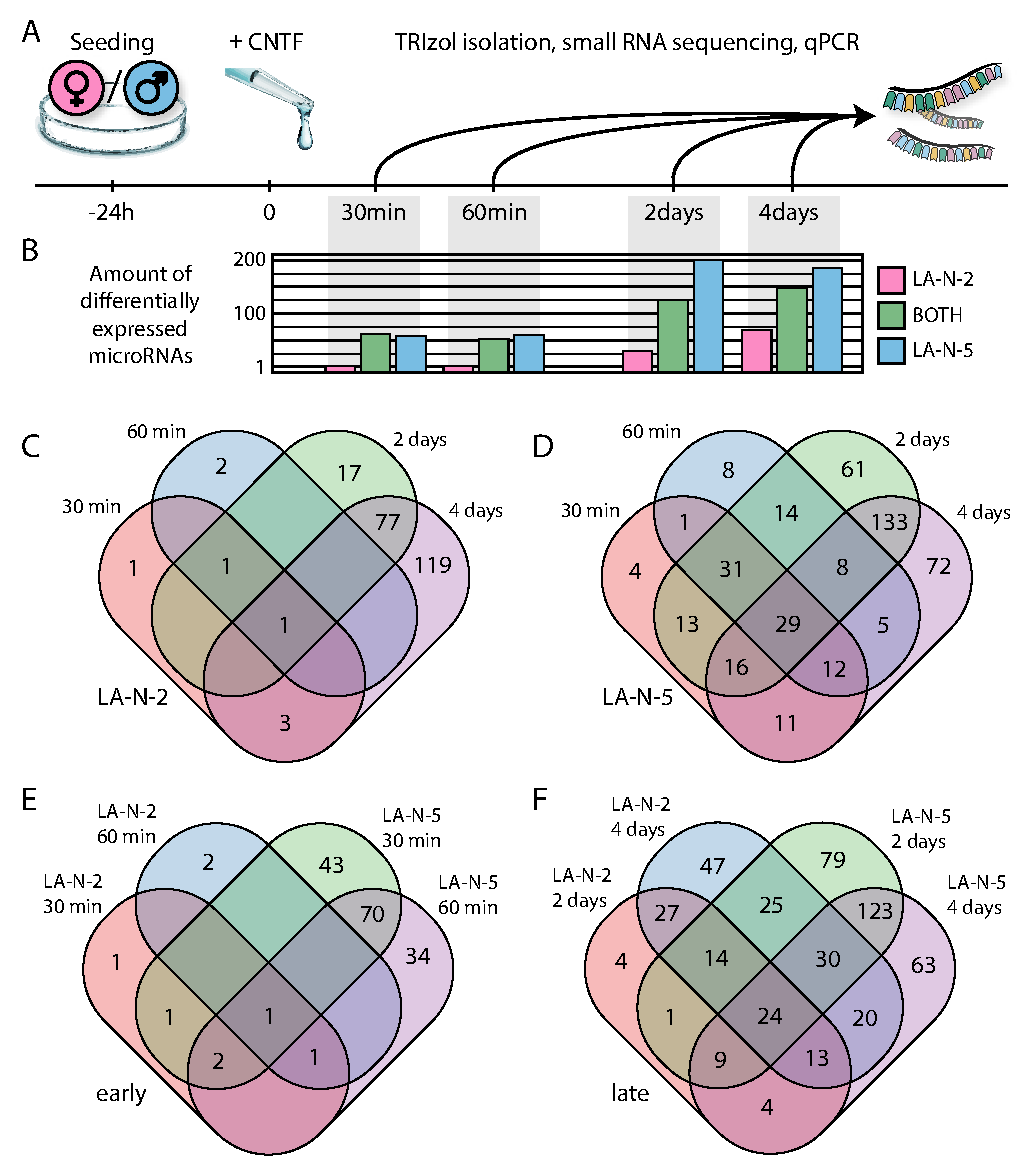
\includegraphics[width=\textwidth]{figures/timepoints-expr-venn}
\caption[Timeline Differential Expression.]{\textbf{LA-N-2 / LA-N-5 Timeline and Differential Expression.} \textbf{A)} Experimental timeline of CNTF differentiation. \textbf{B)} Bar plot of \acf{de} \acp{mir} per time point, divided by cell line where differential expression was measured (\ac{la2} only, \ac{la5} only, or both). \textbf{C)} Venn diagram of \ac{de} \acp{mir} in \ac{la2}, divided by time point. Few early \ac{de} miRNAs, and continually more the longer differentiation lasts. \textbf{D)} Venn diagram of \ac{de} miRNAs in \ac{la5}, divided by time point. Similar in pattern to \textbf{C}, but more pronounced in number. \textbf{E)} Intersection of early time points in \ac{la2} and \ac{la5}. Despite the low differential expression in \ac{la2}, there is overlap. \textbf{F)} Intersection of late time points in \ac{la2} and \ac{la5}. Overlap is pronounced and complex, however, there are also cell line exclusive \acp{mir}.
\label{fig:timepoints-expr-venn}}
\end{figure}

\subsubsection{Differential Expression Between LA-N-2 and LA-N-5}
While there was considerable intersection in \ac{de} \acp{mir} between the cell lines, a substantial amount of \acp{mir} was only \ac{de} in one of the two lines. Generally, response to \ac{cntf} was higher in the male-originated \ac{la5} cells; however, there were also \acp{mir} found \ac{de} only in the female \ac{la2} (compare Fig.\,\ref{fig:timepoints-expr-venn}). Thus, not all of the differences in \ac{mir} expression can be attributed to a higher sensitivity in \ac{la5}. Similarly, \ac{la5} shows a »non-significant trend« toward higher count-change values (mean of absolute count-change across all DE time points, \num{20907} versus \num{3066}, Welch two-sample t test, p = 0.08).

The influence of genotype on the differentiating effect of \ac{cntf} was determined via a statistical interaction design in the \textit{DESeq2} Wald test. Briefly, by including an interaction term in the linear regression formula, the effect of the condition (\ac{cntf} or control at each time point) between the two genotypes can be isolated: $$y \smallsim condition + genotype + condition:genotype$$

Using the interaction term $condition:genotype$, \acp{mir} that reacted significantly different to \ac{cntf} stimulation in \ac{la5} compared to \ac{la2} were determined. Of note, the sexual dimorphism becomes more pronounced over the course of differentiation. While there is no significant difference between \ac{la2} and \ac{la5} at 30 minutes and only one \ac{mir} \ac{de} at 60 minutes, numbers increase at 2 days and reach a maximum at 4 days, with significant overlap (Fig.\,\ref{fig:la2-vs-la5-overlap-venn}\,A). Although not all miRNAs found in this manner belong to the group of miRNAs with inverted expression between LA-N-2 and LA-N-5, several show significant differential regulation between the male and female cellular models (e.g., hsa-miR-615-3p, Fig.\,\ref{fig:la2-vs-la5-overlap-venn}\,B). To further examine the effect of genotype on the small RNA response to \ac{cntf}, the regular differential expression results (Section \ref{sec:cellculture:along}) were intersected with the interaction term for the late time points. This resulted in a complex pattern of intersecting \acp{mir}, in both cell lines (Fig.\,\ref{fig:la2-vs-la5-overlap-venn}\,C\&D). Again, all possible overlaps between any two groups exist; 37 and 36 \acp{mir} are found in all four groups of \ac{la2} and \ac{la5}, respectively. Among those, 16 mature \acp{mir} belong to all sets. All pertinent sets of \acp{mir} can be found in Appendix \ref{appendix:de-mirs}. \todo{target, GO for which?}

\begin{figure}
\centering
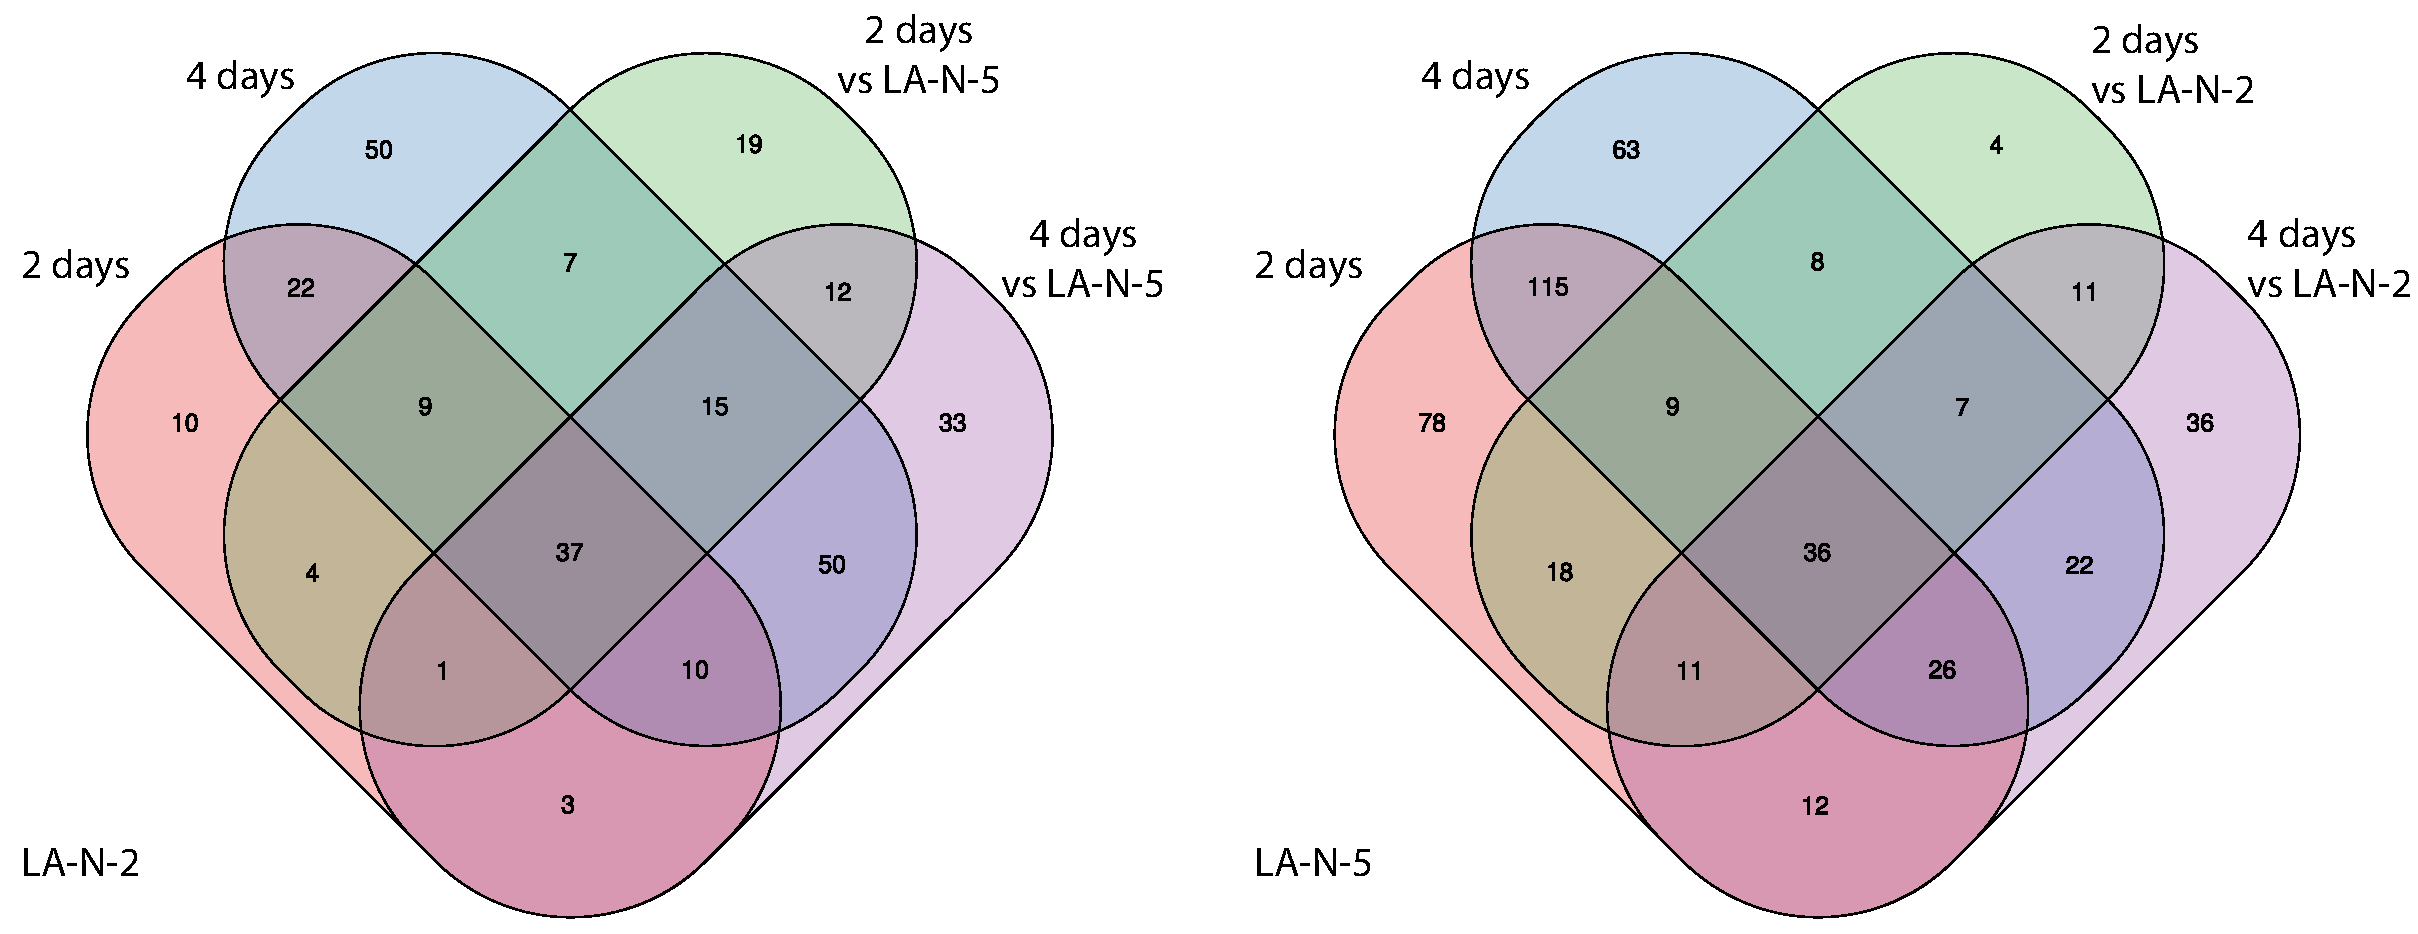
\includegraphics[width=\textwidth]{figures/la2-vs-la5-overlap-venn}
\caption[miRNAs DE between LA-N-2 and LA-N-5.]{\textbf{miRNAs DE between LA-N-2 and LA-N-5.} Application of a design model formula which includes an interaction term enables display of the influence of the male or female genotype on differential miRNA expression. \textbf{A)} Venn diagram of miRNAs differentially expressed \emph{between} LA-N-2 and LA-N-5 at all four time points. \textbf{B)} Counts plot of normalised raw expression values of hsa-miR-615-3p. Exemplary of a high influence of genotype on the differential expression caused by CNTF differentiation, hsa-miR-615-3p is more highly expressed in the female LA-N-2 and elevated after four days of CNTF-induced differentiation, while in the male LA-N-5, it is expressed slightly lower and suppressed upon differentiation. \textbf{C)} Venn diagram comparing late differential expression in LA-N-2 with late time points of differential expression between LA-N-2 and LA-N-5. All possible combinations exist, however, there are miRNAs affected by genotype that are not differentially expressed in the simple model. \textbf{D)} Venn diagram comparing late differential expression in LA-N-5 with late time points of differential expression between LA-N-2 and LA-N-5. Essentially similar to C), but with partly higher quantities of DE miRNAs.
\label{fig:la2-vs-la5-overlap-venn}}
\end{figure}

\subsection{microRNA Family Enrichment}
To categorise and systematise the sexual dimorphism of \ac{cntf} differentiation of LA-N cells, statistically over-represented \ac{mir} families in the differential expression datasets were determined.\todo{how many DE miRs in families?} Of the 151 \ac{mir} families listed in miRBase v21, members of 71 families are \ac{de} in \ac{la2} and \ac{la5}. Enrichment of male, female, and ubiquitously \ac{de} \acp{mir} in these families was determined via hypergeometric gene set enrichment based on Fisher's exact test for each of the families. Five families were enriched in both male and female cells, and 12 families in only one of the two cell lines (Fig.\,\ref{fig:mir-de-fam-go}\,A, left side). The size range of enriched families was substantial, from small families with only 4 mature members to extensive families with dozens of mature \acp{mir}. \todo{which/how many of the pertinent mirs above are in families?}

\subsubsection{Gene Targeting of Enriched Families}
The targets of all individual \acp{mir} in the enriched families were determined via \textit{miRNetDB} query. Of note, the amount of family members in any \ac{mir} family did not correlate with the absolute amount of targets predicted (Fig.\,\ref{fig:mir-de-fam-go}\,A). Rather, the influence of individual \acp{mir} was the main factor determining the size of the gene target network. However, those families that were enriched in only one cell line presented with significantly smaller target sets than those that were found \ac{de} in both (mean targeted genes per \ac{mir} 217 versus 378, Welch two-sample t test, p = 0.001). Relative to family size, 4 of the enriched families targeted less genes than all others: mir-10 (p = 0.016), mir-192 (p = 0.042), mir-379 (p = 0.011), and mir-515 (p < 0.001). Hypothetically, the spectrum of target amounts may correlate with the degree of functional specification of distinct \ac{mir} families: on one end, broadly acting families such as let-7 with sex-independent function, on the other, families with a narrow target profile, such as mir-10, whose restricted function can associate with sex-specific effects.

\begin{figure}
\centering
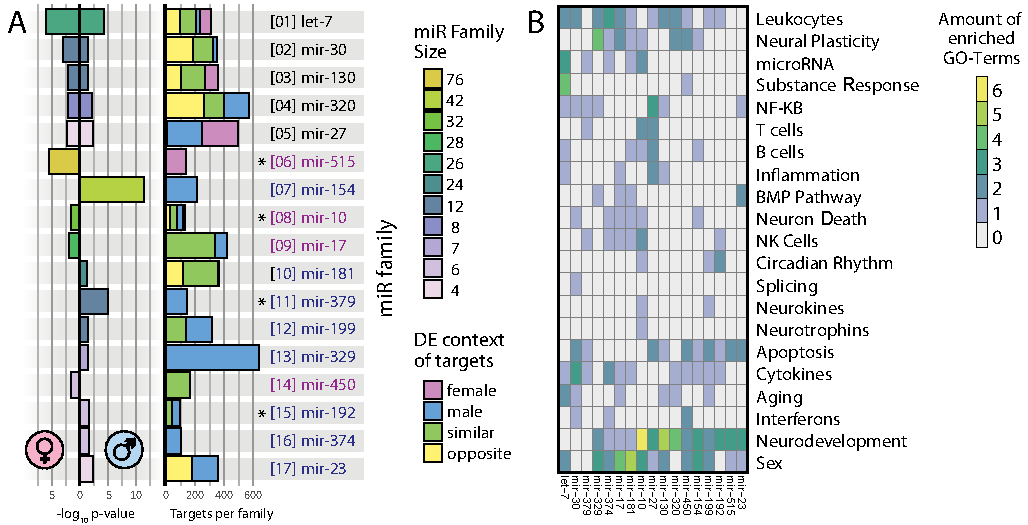
\includegraphics[width=\textwidth]{figures/mir-de-fam-go}
\caption[Differential Expression miRNA Family Enrichment]{\textbf{miRNA Families Enriched in Differential Expression and their Ontological Associations.} 17 miRNA families were enriched significantly in the DE miRNAs following CNTF-mediated differentiation of LA-N-2 and LA-N-5 (Fisher's exact test, p < 0.05). \textbf{A, left side)} Bar plot of p-values of enriched families, ordered by family size; family size encoded by colour. \textbf{A, right side)} Stacked bar plot of the number of gene targets per family. Bars are divided by the DE pattern between LA-N-2 and LA-N-5 of each individual family member. DE context (encoded by colour) varies from detection in all categories (such as let-7 or mir-10) to detection only in one cell line (such as mir-515 or mir-154). Four families show significantly less target genes than all other families in relation to their size (denoted by asterisks). \textbf{B)} Gene Ontology enrichment analysis of gene targets of all enriched families, 737 distinct terms curated into CNS- or immunity-related categories. Families mir-10 and mir-199 show association with neurokines and circadian rhythm.
\label{fig:mir-de-fam-go}}
\end{figure}